\documentclass{article}

\usepackage{tikz}
\usetikzlibrary{calc}
\begin{document}
\begin{figure}
\tikzset{
tick/.style = {black, very thick}
}

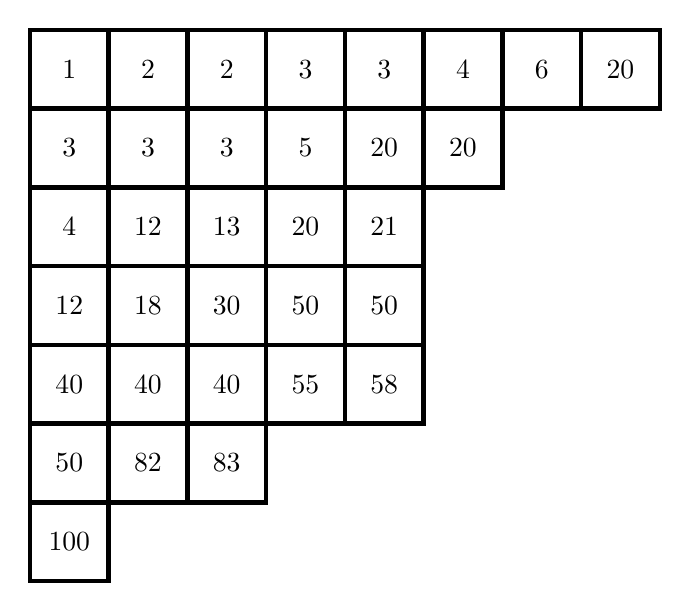
\begin{tikzpicture} % boxlength=1%ZEILE NR. 0 (von unten)

%ELEMENT IN SPALTE NR. 0 (von links)
\draw [ultra thick] (0,0) rectangle (1,1);
\node at ($(0.5,0.5)$) {$100$};




%ZEILE NR. 1 (von unten)

%ELEMENT IN SPALTE NR. 0 (von links)
\draw [ultra thick] (0,1) rectangle (1,2);
\node at ($(0.5,1.5)$) {$50$};

%ELEMENT IN SPALTE NR. 1 (von links)
\draw [ultra thick] (1,1) rectangle (2,2);
\node at ($(1.5,1.5)$) {$82$};

%ELEMENT IN SPALTE NR. 2 (von links)
\draw [ultra thick] (2,1) rectangle (3,2);
\node at ($(2.5,1.5)$) {$83$};




%ZEILE NR. 2 (von unten)

%ELEMENT IN SPALTE NR. 0 (von links)
\draw [ultra thick] (0,2) rectangle (1,3);
\node at ($(0.5,2.5)$) {$40$};

%ELEMENT IN SPALTE NR. 1 (von links)
\draw [ultra thick] (1,2) rectangle (2,3);
\node at ($(1.5,2.5)$) {$40$};

%ELEMENT IN SPALTE NR. 2 (von links)
\draw [ultra thick] (2,2) rectangle (3,3);
\node at ($(2.5,2.5)$) {$40$};

%ELEMENT IN SPALTE NR. 3 (von links)
\draw [ultra thick] (3,2) rectangle (4,3);
\node at ($(3.5,2.5)$) {$55$};

%ELEMENT IN SPALTE NR. 4 (von links)
\draw [ultra thick] (4,2) rectangle (5,3);
\node at ($(4.5,2.5)$) {$58$};




%ZEILE NR. 3 (von unten)

%ELEMENT IN SPALTE NR. 0 (von links)
\draw [ultra thick] (0,3) rectangle (1,4);
\node at ($(0.5,3.5)$) {$12$};

%ELEMENT IN SPALTE NR. 1 (von links)
\draw [ultra thick] (1,3) rectangle (2,4);
\node at ($(1.5,3.5)$) {$18$};

%ELEMENT IN SPALTE NR. 2 (von links)
\draw [ultra thick] (2,3) rectangle (3,4);
\node at ($(2.5,3.5)$) {$30$};

%ELEMENT IN SPALTE NR. 3 (von links)
\draw [ultra thick] (3,3) rectangle (4,4);
\node at ($(3.5,3.5)$) {$50$};

%ELEMENT IN SPALTE NR. 4 (von links)
\draw [ultra thick] (4,3) rectangle (5,4);
\node at ($(4.5,3.5)$) {$50$};




%ZEILE NR. 4 (von unten)

%ELEMENT IN SPALTE NR. 0 (von links)
\draw [ultra thick] (0,4) rectangle (1,5);
\node at ($(0.5,4.5)$) {$4$};

%ELEMENT IN SPALTE NR. 1 (von links)
\draw [ultra thick] (1,4) rectangle (2,5);
\node at ($(1.5,4.5)$) {$12$};

%ELEMENT IN SPALTE NR. 2 (von links)
\draw [ultra thick] (2,4) rectangle (3,5);
\node at ($(2.5,4.5)$) {$13$};

%ELEMENT IN SPALTE NR. 3 (von links)
\draw [ultra thick] (3,4) rectangle (4,5);
\node at ($(3.5,4.5)$) {$20$};

%ELEMENT IN SPALTE NR. 4 (von links)
\draw [ultra thick] (4,4) rectangle (5,5);
\node at ($(4.5,4.5)$) {$21$};




%ZEILE NR. 5 (von unten)

%ELEMENT IN SPALTE NR. 0 (von links)
\draw [ultra thick] (0,5) rectangle (1,6);
\node at ($(0.5,5.5)$) {$3$};

%ELEMENT IN SPALTE NR. 1 (von links)
\draw [ultra thick] (1,5) rectangle (2,6);
\node at ($(1.5,5.5)$) {$3$};

%ELEMENT IN SPALTE NR. 2 (von links)
\draw [ultra thick] (2,5) rectangle (3,6);
\node at ($(2.5,5.5)$) {$3$};

%ELEMENT IN SPALTE NR. 3 (von links)
\draw [ultra thick] (3,5) rectangle (4,6);
\node at ($(3.5,5.5)$) {$5$};

%ELEMENT IN SPALTE NR. 4 (von links)
\draw [ultra thick] (4,5) rectangle (5,6);
\node at ($(4.5,5.5)$) {$20$};

%ELEMENT IN SPALTE NR. 5 (von links)
\draw [ultra thick] (5,5) rectangle (6,6);
\node at ($(5.5,5.5)$) {$20$};




%ZEILE NR. 6 (von unten)

%ELEMENT IN SPALTE NR. 0 (von links)
\draw [ultra thick] (0,6) rectangle (1,7);
\node at ($(0.5,6.5)$) {$1$};

%ELEMENT IN SPALTE NR. 1 (von links)
\draw [ultra thick] (1,6) rectangle (2,7);
\node at ($(1.5,6.5)$) {$2$};

%ELEMENT IN SPALTE NR. 2 (von links)
\draw [ultra thick] (2,6) rectangle (3,7);
\node at ($(2.5,6.5)$) {$2$};

%ELEMENT IN SPALTE NR. 3 (von links)
\draw [ultra thick] (3,6) rectangle (4,7);
\node at ($(3.5,6.5)$) {$3$};

%ELEMENT IN SPALTE NR. 4 (von links)
\draw [ultra thick] (4,6) rectangle (5,7);
\node at ($(4.5,6.5)$) {$3$};

%ELEMENT IN SPALTE NR. 5 (von links)
\draw [ultra thick] (5,6) rectangle (6,7);
\node at ($(5.5,6.5)$) {$4$};

%ELEMENT IN SPALTE NR. 6 (von links)
\draw [ultra thick] (6,6) rectangle (7,7);
\node at ($(6.5,6.5)$) {$6$};

%ELEMENT IN SPALTE NR. 7 (von links)
\draw [ultra thick] (7,6) rectangle (8,7);
\node at ($(7.5,6.5)$) {$20$};







\end{tikzpicture}
\end{figure}
\end{document}

